In order to have a better idea of the performances of the DBC regarding the bandwidth of the signal, simulation of the retrieved visibilities and phases have been ran. To do that the simulated polychromatic light is injected into 2 of the 4 inputs. At one of the input a phase is added just the same as for constructing the V2PM. At each output an interferogram is reconstructed showing the visibility function versus the OPD. These interferogram (in the shape of a matrix where each column is one simulated phase of the \gls{bl}) are multiplied by the P2VM to obtain the $\vec{V}$ vector from which the object visibility are calculated as explained in sections \ref{sec:mathmono} and \ref{sec:mathpoly}. The results are presented in Fig.\ref{fig:retrieved_nofan} and Fig.\ref{fig:retrieved_fan}

In our simulation no polarization's effects are taken into account so that the visibility of the input source should be 1 at the 0 OPD independently of the phase difference. All simulations were performed with one data point each 12 degrees of phase difference between the inputs from 0 to 360 degrees, for all 50 wavelength evenly spaced in a fixed bandwidth around 3.4 µm and for all 6 baselines. 

To estimate the accuracy of the retrieved phases and visibilities, the expected ones are subtracted from the retrieved ones and the deviation $\epsilon$ is estimated by the formula :
\begin{equation}\label{eq:deviation}
\epsilon = \sqrt{\frac{1}{N}\sum_{1}^{N}(a-\Tilde{a})^2}
\end{equation}

where $a$ is the retrieved parameters, $\Tilde{a}$ the expected one and $N$ the number of tested retrieved parameters (31 in out case).
The result is shown in Fig \ref{fig:retrieved_nofan}. What can be seen is that the retrieved visibilities are close to the expected ones (at $\pm5\%$ for bandwidth below 60 nm bandwidth), same as the retrieved phases (at $\pm 0.05 rad$ below 60 nm bandwidth).
Meanwhile the standard deviation of both the retrieved phases and visibilities are found to have a similar dependency to the bandwidth. This means that the larger the bandwidth, the more dispersed the retrieved parameters around their mean value. 
The results for the component with a "fan-out" is very similar as can be seen in Fig. \ref{fig:retrieved_fan} despite a lower condition number of the V2PM. This clearly shows that the condition number only states the maximum magnification of an error. It also shows that despite the apparent correlation between the retrieved visibilities/phases and the condition number of the V2PM, the impact of this condition number is not the main limiting factor but the approximations of "flat spectral response" is. The broader the bandwidth the more the spatial frequency of the interferogram (i.e the fringe spacing) can get different from 3.4 \si{\micro\meter}. 


\begin{figure}[htbp]
    \centering
    \begin{subfigure}{.45\textwidth}
        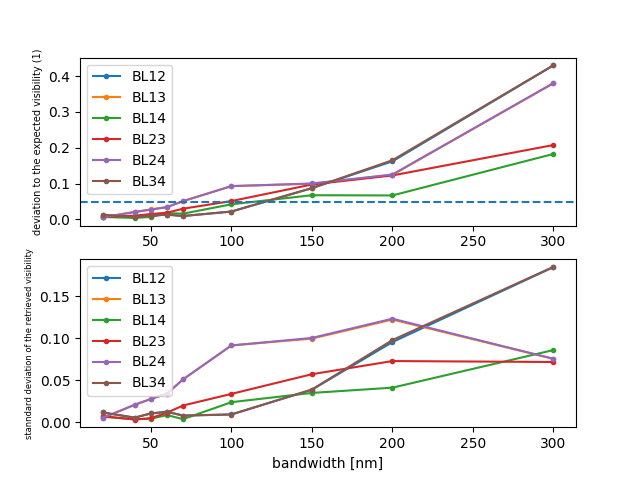
\includegraphics[scale=.45]{picture/retrieval_simu/visi_retrieved_nofan.png}
        \caption{Deviation of the retrieved visibilities to the expected ones}
    \end{subfigure}%
    \begin{subfigure}{.45\textwidth}
    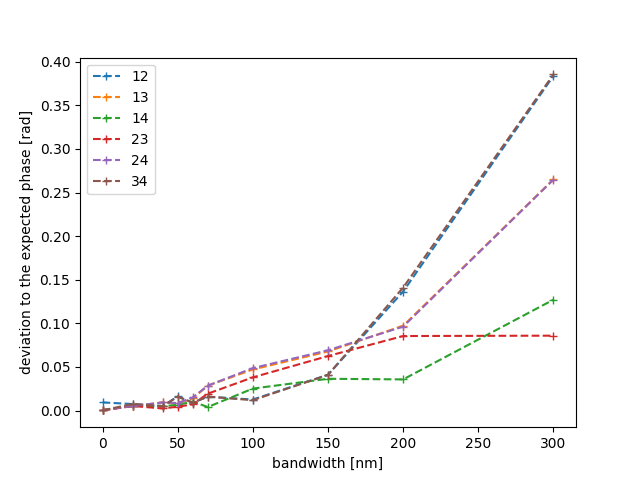
\includegraphics[scale=.45]{picture/retrieval_simu/phase_retrieved_nofan.png}
    \caption{Deviation of the retrieved phases to the expected ones}
    \end{subfigure}
    \caption{Deviation of the retrieved phases and visibilities to the expected ones for the component without fan-out. The deviation is calculated by Eq. \ref{eq:deviation}}. In order to compare with the experimental results presented in the following part, the plots of the retrieved visibility and phases with 70nm bandwidth are presented in Appendix \ref{an:retriev}
    \label{fig:retrieved_nofan}
\end{figure}

\begin{figure}[htbp]
    \centering
    \begin{subfigure}{.45\textwidth}
        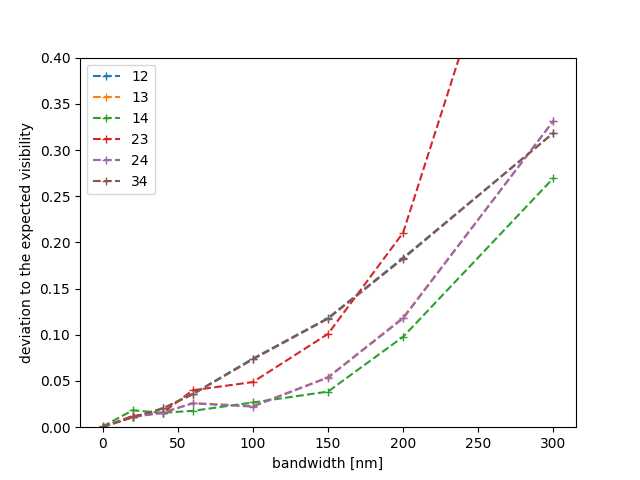
\includegraphics[scale=.45]{picture/retrieval_simu/visi_retrieved_fan.png}
        \caption{Deviation  of the retrieved visibilities to the expected ones}
    \end{subfigure}%
    \begin{subfigure}{.45\textwidth}
    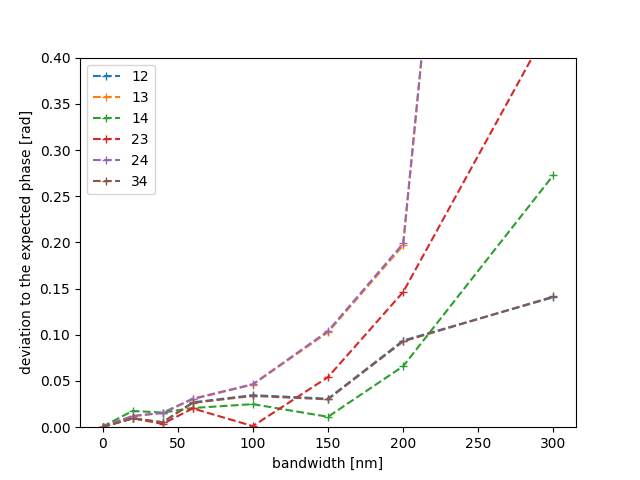
\includegraphics[scale=.45]{picture/retrieval_simu/phase_retrieved_fan.png}
    \caption{Deviation of the retrieved phases to the expected ones}
    \end{subfigure}
    \caption{Deviation of the retrieved phases and visibilities to the expected ones for the component with fan-out. The deviation is calculated by Eq. \ref{eq:deviation}. The blue dashed line is the limit of 5\% error. Inputs 1,2,3,4 refers respectively to WG 19,14,10,5 in Fig.\ref{tikz:ZigZagCrossSection} as seen from the inputs.}
    \label{fig:retrieved_fan}
\end{figure}

From the results of these simulation, an experimental demonstration of the usability of the DBC with a signal of 70nm bandwidth is still to be done. This is the purpose of the next chapter.
